\newpage

\section{Integrating Acceleration}

\subsection{Parts List}

\begin{enumerate}[itemsep=-5pt]
\item CPX/CPB
\item USB Cable
\item Laptop
\item Some sort of temporary adhesive
\item Automobile
\end{enumerate}

\subsection{Learning Objectives}
\begin{enumerate}[itemsep=-5pt]
\item Taking acceleration data of real systems
\item Numerical Integration 
\item The dangers of integration bias
\end{enumerate}

\subsection{Getting Started}

The code for this lab is to have the CPX log acceleration. So when you’re done with this lab you will hopefully have a data file with 4 columjns of data: time, acceleration x, acceleration y, acceleration z. The code I’m using is the same as the lab on accelerometers (See chatper \ref{s:modules}). I’m using method 1 for datalogging so I’m just having it print to Serial (See chapter \ref{s:daq}).
\begin{figure}[H]
  \begin{center}
    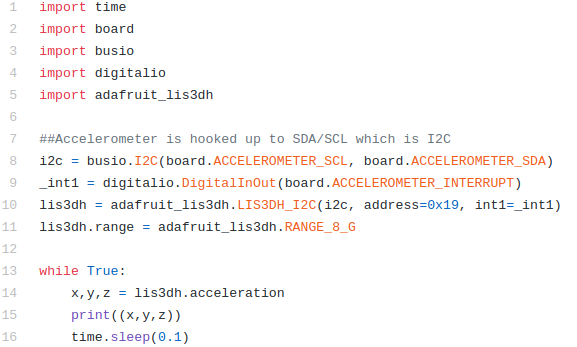
\includegraphics[width=0.8\textwidth]{Figures/accelerometer_code1.png}
  \end{center}
\end{figure}
The code on Github has a sleep of 0.1 seconds but make sure to have the CPX take data as fast as possible. A sleep of 0.01 is probably good. You will probably get a lot of data points for this experiment. Once your code is working, place the CPX on your dashboard with one of the axes of the accelerometer pointing towards the nose of your car. Try and place the CPX on as flat a surface as possible. You can use 3M tape or duct tape or hot glue. Just make sure you don’t damage your car and make sure the CPX is well anchored to the dashboard. This way when the car accelerates, the CPX will measure that acceleration. Note, if you’d like to do this with a bike or some other motor vehicle that is just fine. Just make sure to take pictures and videos when you do the experiment. I suggest you do this in a parking lot for safety reasons. I am not responsible for any damage done to your vehicle or anyone else because you are doing this project. Once you have the CPX anchored, accelerate your vehicle to 20 mph (or however fast you are comfortable driving) and then slam on the brakes. Once your data is logged, plot your acceleration in Python on your desktop computer. After doing the experiment myself, this is what my acceleration plot looks like. I had to clip the time series to only include the part from where I accelerated and decelerated quickly. I also subtracted the first data point from each accelerometer axis to zero it out and subtract off the bias. Since I took some data for a bit before I started moving I could have averaged the first few data points to obtain the bias. \href{https://www.youtube.com/watch?v=e4xs9Ky7_YI&feature=youtu.be}{I’ve done this in a Youtube video if you’re unsure what I mean}. Instead just to get something working properly I went ahead and just used the first data point.
\begin{figure}[H]
  \begin{center}
    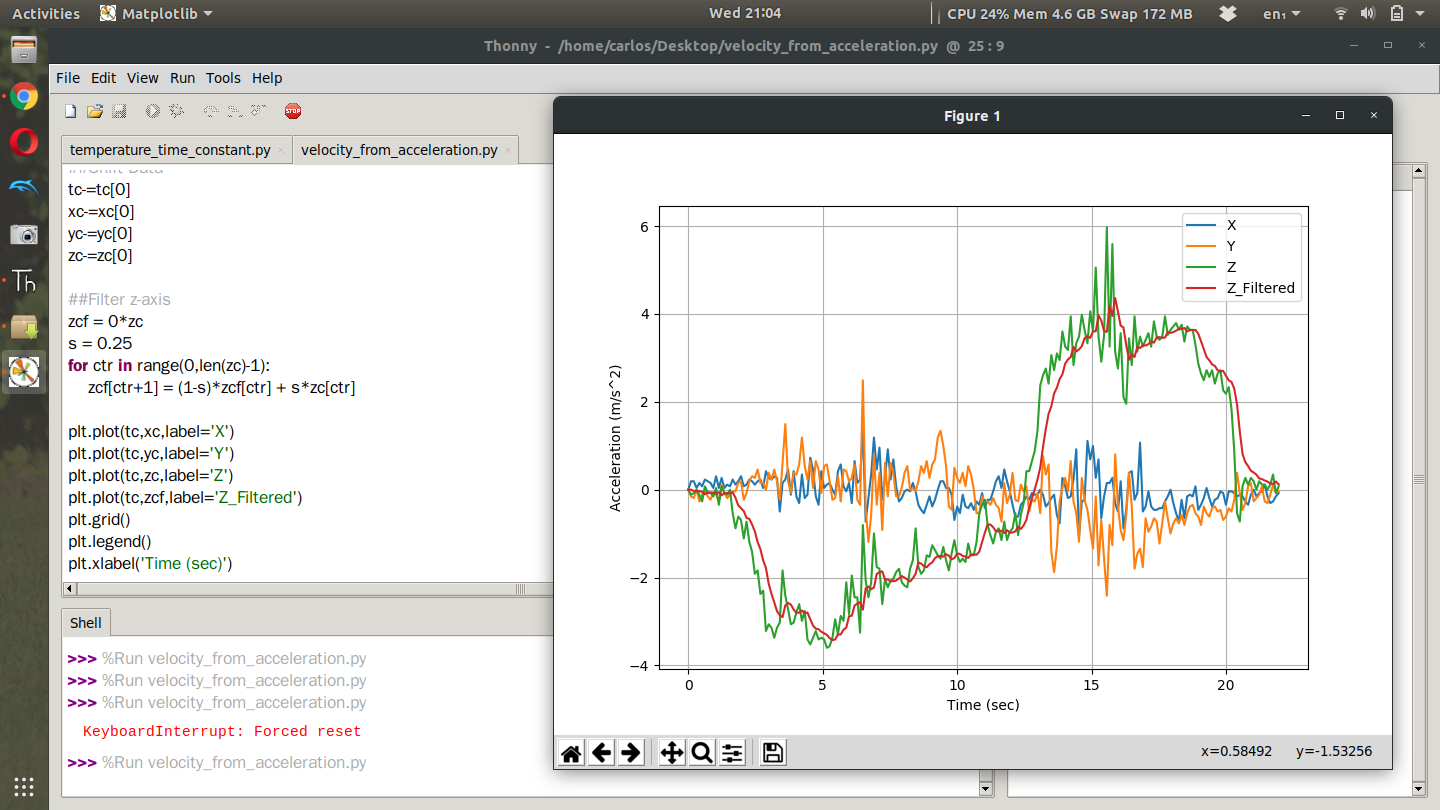
\includegraphics[width=\textwidth]{Figures/accelerometer_plots.png}
  \end{center}
\end{figure}
It’s clear from the plots that the z axis was oriented towards the nose of the car. In this case I am going to have to flip the z-axis since the beginning is acceleration and the end is deceleration. I also through the acceleration in the z-axis through a complementary filter with a filter value of 0.25. I think it makes the acceleration profile a bit less jumpy. I then used a Reimann sum and integrated the acceleration data points to get velocity. The equation itself looks like this:
\begin{equation}
V_i = \sum\limits_{n=0}^{i}{(a_i-a_0)\Delta t}
\end{equation}
This of course assumes the initial velocity is zero. Notice that I take the individual acceleration points and subtract off the bias. Computing that summation by hand is pretty trivial but getting the code to work is another story. For a Reimann sum we’re going to use a for loop where we loop through all the data points. The good news is that the time between data points is the same so we can just treat that as a constant. Once you have acceleration integrated you can plot velocity. This is what mine looks like after I did the experiment. According to my plot I accelerated to about 45 mph. I guess I can’t lie in this instance. I said to accelerate to 20 mph but I really wanted to see a large change in acceleration so I punched it. Notice though that at the end of the time series the velocity is negative. This is because as time goes on you are integrating error and the error just gets worse.
\begin{figure}[H]
  \begin{center}
    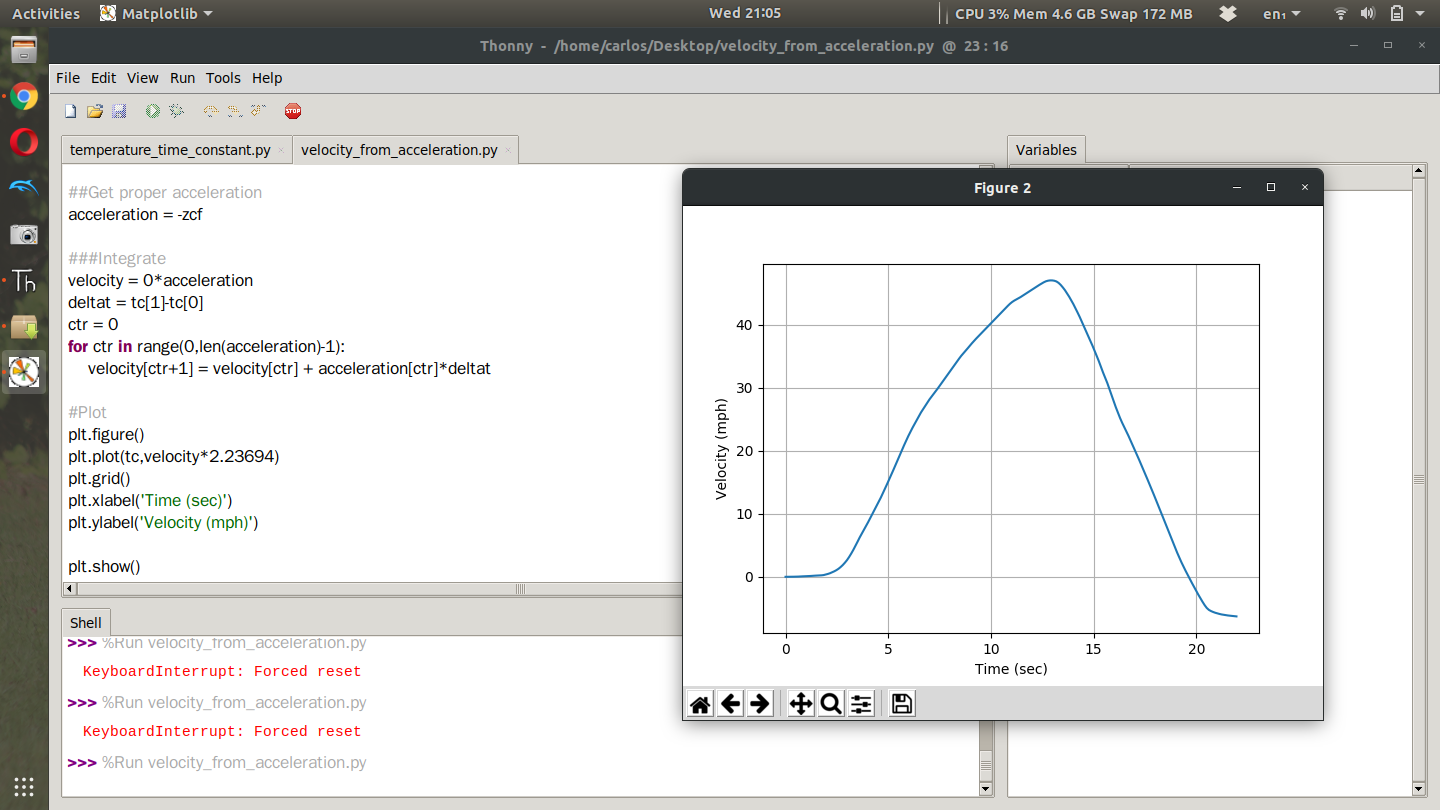
\includegraphics[width=\textwidth]{Figures/accelerometer_integration.png}
  \end{center}
\end{figure}
This is why speedometers are used. They are just much more accurate than integrating acceleration which is prone to bias and drift. \href{https://github.com/cmontalvo251/Python/tree/master/instrumentation/cpx_assignments/Velocity_from_Acceleration}{This folder on Github has some codes that will help with your project}. {\bf Note, that some of those codes have a bias filter, truncation filter and complementary filter. That code may not work for you and you may need to tune the filters for your specific data set. Make sure to understand what each filter does and think about how it applies to your data set otherwise your code may throw an error due to the differences in your data set.}

\subsection{Assignment}

For this assignment you are to find a safe place to accelerate and decelerate your vehicle while recording acceleration. I suggest using a temporary adhesive to secure your CPX/CPB to your dashboard (making sure it's level) and have a passenger in the car to help you record data. Again for safety's sake I suggest finding an empty parking lot and only accelerating to 20 mph or less.

Once you've completed the project above, upload a PDF with all of the photos and text
below included. My recommendation is for you to create a Word document
and insert all the photos and text into the document. Then export the
Word document to a PDF. For videos I suggest uploading the videos to
Google Drive, turn on link sharing and include a link in your
PDF. Note that all code must be included in the appendix or you'll be
penalized 10\%. 


\begin{enumerate}[itemsep=-5pt]
\item Include a picture of your car and your passenger that is helping you record data. In your description write what speed you achieved in your experiment. - 10\%
\item Include a photo of your CPX/CPB mounted to your vehicle indicating which axis of acceleration is pointing forward - 10\%
\item Plot one axis of your accelerometer data vs time which clearly indicates when you accelerated and decelerated. In your description be sure to explain which axis you are plotting and any signal conditioners you applied to get your clean signal - 20\%
\item Integrate acceleration and plot velocity as a function of time. Comment on whether or not the maximum velocity is the same as what you did in your actual car - 20\%
\item Integrate the velocity and compute position. Plot your position as a function of time and include that in your report. Although you didn't measure how far you went, comment on the accuracy of the plot and whether or not you think you traveled that far - 20\%
\end{enumerate}
